\subsection{تست نرم افزار}

فرایند تست نرم افزار در حین توسعه محصول انجام می‌گیرن. مدلی که استفاده می‌کنیم، TDD خواهد بود. در هر مرحله از پیاده سازی نرم افزار، محصول تست می‌شود.

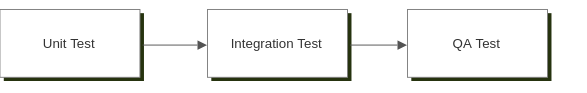
\includegraphics[scale=1]{assets/testing_DFD.png}

\subsubsection{تست واحد نرم افزار}

در حین توسعه هر زیر سیستم، نیاز به نوشتن یک سری تست واحد برای مطمعن شدن از درست کار کردن هر تابع یا کلاس خواهد بود. این تست ها در سورس کد هستند 
و در فرایند CI تعیین می‌شود که هیچ PR مرج نمی‌شود، اگر اینکه تمام تست های آن پاس شده باشد.
درواقع سیستم خودکار ما ابتدا بواسطه pipeline هایی که باید تست های واحد را چک می‌کند و اگر پاس شدند به مرحله بعد می‌رود.

\subsubsection{تست جامعیت}

پس از تکمیل تمامی سیستم ها، زیر سیستم ها کنار هم قرار گرفته و نیاز به تست Integration یا جامعین وجود خواهد داشت.
برای این کار ابزار های متنوعی وجود دارد. تیم ما از ابزار Postmanاستفاده می‌کند و در نهایت، داخل سرور CI
از newman استفاده می‌کند تا بتواند کالکشن های توسعه داده شده را با داده های تستی در سرور برای هر PR امتحان کند. این نیازمند این هست که اول اپلیکیشن به صورت خودکار در سرور تستی لانچ شود.

\subsubsection{تست پذیرش}

برای این موضوع تحلیل گران و تیم QA وارد کار می‌شوند. واحد کنترل کیفیت باید تمام اجزای UI و عملکرد سیستم را برسی کند و اطمینان حاصل کند که مشکل وجود ندارد و همه چیز بر اساس دیزاین درست کار می‌کند.
